\documentclass{article}

%\usepackage{INTERSPEECH2019}
\usepackage{spconf}

\usepackage{graphicx}
\usepackage{amssymb,amsmath,bm}
\usepackage{textcomp}
%\usepackage{spconf,amsmath,graphicx,amssymb,epsfig, graphicx, url}
\usepackage[tight,footnotesize]{subfigure}
\usepackage{url}
\def\vec#1{\ensuremath{\bm{{#1}}}}
\def\mat#1{\vec{#1}}

\renewcommand{\topfraction}{1.0}
\renewcommand{\bottomfraction}{1.0}
\renewcommand{\textfraction}{0.01}
\renewcommand{\floatpagefraction}{1.0}
\renewcommand{\dbltopfraction}{1.0}
\renewcommand{\floatpagefraction}{1.0}  % require fuller float pages
\renewcommand{\dblfloatpagefraction}{1.0} % require fuller float pages

\newcommand{\etal}{\emph{et al.} }
\newcommand{\eg}{\emph{e.g.} }
\newcommand{\ie}{\emph{i.e.} }


\sloppy % better line breaks
\ninept

\title{Sound Source Separation Using Inter-Microphone Delay, Cross-Correlation,
and Cross-Covariance}

%%%%%%%%%%%%%%%%%%%%%%%%%%%%%%%%%%%%%%%%%%%%%%%%%%%%%%%%%%%%%%%%%%%%%%%%%%
%% If multiple authors, uncomment and edit the lines shown below.       %%
%% Note that each line must be emphasized {\em } by itself.             %%
%% (by Stephen Martucci, author of spconf.sty).                         %%
%%%%%%%%%%%%%%%%%%%%%%%%%%%%%%%%%%%%%%%%%%%%%%%%%%%%%%%%%%%%%%%%%%%%%%%%%%
%\makeatletter
%\def\name#1{\gdef\@name{#1\\}}
%\makeatother
%\name{{\em Firstname1 Lastname1, Firstname2 Lastname2, Firstname3 Lastname3,}\\
%      {\em Firstname4 Lastname4, Firstname5 Lastname5, Firstname6 Lastname6,
%      Firstname7 Lastname7}}
%%%%%%%%%%%%%%% End of required multiple authors changes %%%%%%%%%%%%%%%%%

\makeatletter
\def\name#1{\gdef\@name{#1\\}}
\makeatother \name{{\em Chanwoo Kim$^1$, Anjali Menon$^2$, and Richard M. Stern$^2$\thanks{\textbf{
Thanks to Samsung Electronics for funding this research. The authors are thankful 
to Executive Vice President Seunghwan Cho and speech processing Lab. members at Samsung Research.
}}}}

\address{$^{1}$ Samsung Research \\ $^{2}$ Carnegie Mellon University \\
{\small \tt chanw.com@samsung.com, \{anjalim, rms\}@cmu.edu}}
%
%\twoauthors{Karen Sp\"{a}rck Jones.}{Department of Speech and Hearing \\
%  Brittania University, Ambridge, Voiceland \\
%  {\small \tt Karen@sh.brittania.edu} }
%  {Rose Tyler}{Department of Linguistics \\
%  University of Speechcity, Speechland \\
%  {\small \tt RTyler@ling.speech.edu} }

%
%
\graphicspath{{../figures/}}
%
\newcommand{\chanwcom}{{C. Kim}}
%
\begin{document}
%
  \maketitle
  %
  \begin{abstract}
In this paper, we present a two-microphone algorithm for sound source separation 
    referred to as Minimum Normalized Cross-Correlation and Minimum Normalized 
    Cross-coVariance (MNCC-MNCV).  
    The MNCC-MNCV algorithm automatically selects the ``Inter-Microphone
    Delay (IMD) threshold," which separates time-frequency segments that are believed to
    belong to the target from components that are dominated by noise sources.
    In this work, we develop an algorithm which considers both the
    normalized correlation and the correlation coefficient of the target and
    interfering signal signals, after a compressive nonlinearity. 
We demonstrate that the use of the MNCC-MNCV method of estimating IMD
    thresholds  provides significantly better recognition accuracy in the
    presence of   interfering speech sources, omni-directional noise, and
    reverberation than several other approaches including ZCAE
    \cite{H_Park_SpeechComm_2009}, PDCW \cite{C_Kim_INTERSPEECH_2009_1}, and
    our previous automatic IMD threshold selection approach
    \cite{C_Kim_INTERSPEECH_2010_1}. 
  \end{abstract}
%  
  \noindent{\bf Index Terms}: Robust speech recognition, signal separation, phase difference analysis,  cross-correlation, normalized correlation
%
%
\section{Introduction}
%
\begin{figure*}[t]
            \begin{center}
                    {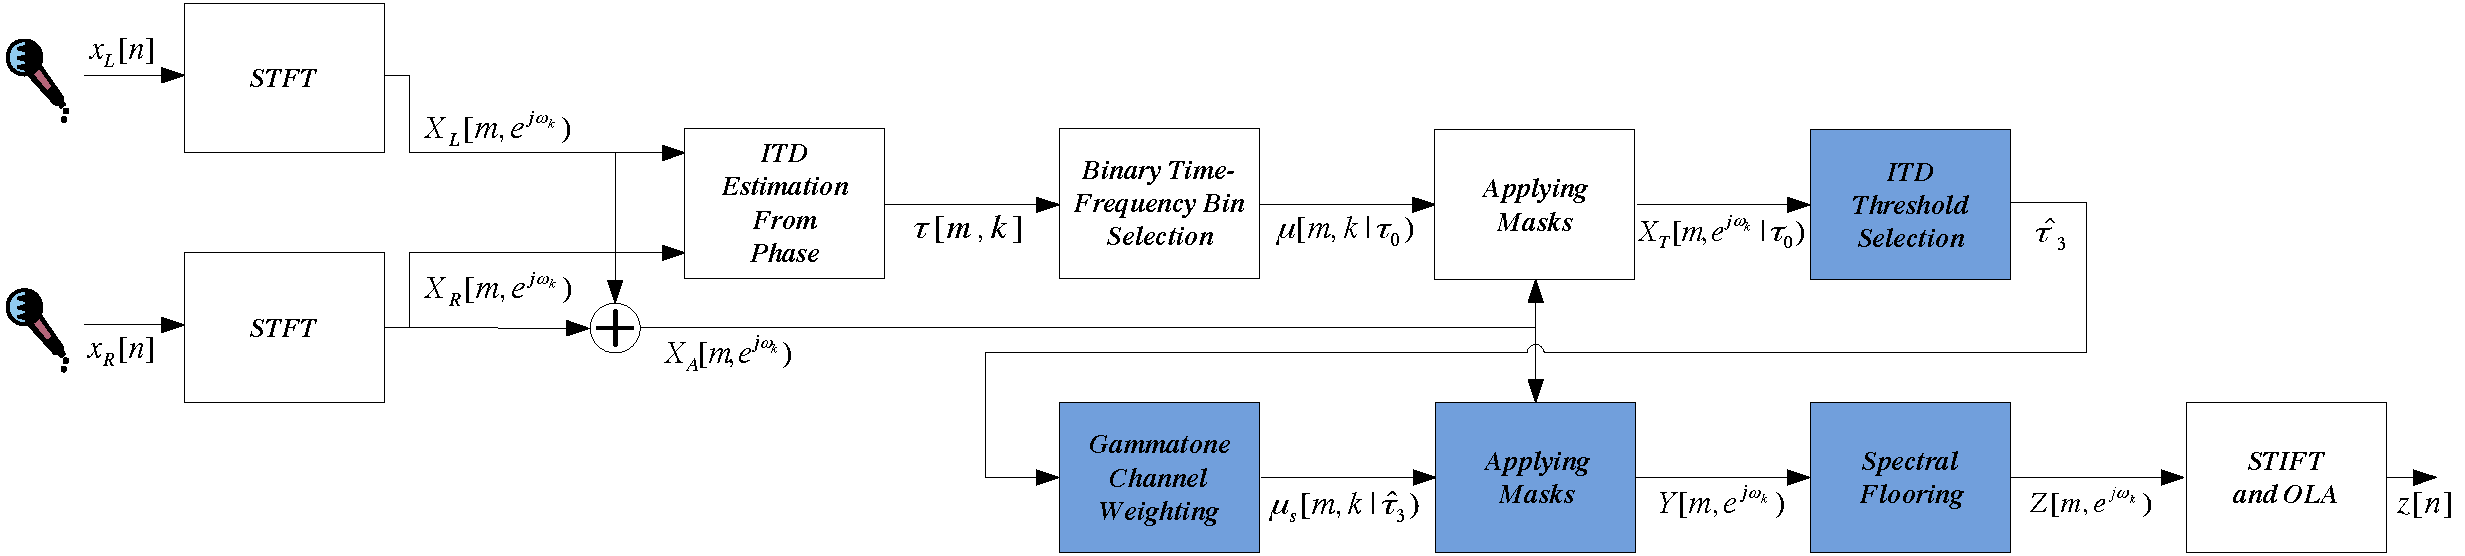
\includegraphics[width=170mm]{../figures/PDCW_AUTO_BlockDiagram}}
            \end{center}
	%\vspace{-6mm}
 \caption{\label{fig:PDCW_AUTO_BlockDiagram}
       \emph{ Block diagram of a sound source separation system using the
       MNCC-MNCV algorithm. }
       }	\vspace{-6mm}
\end{figure*}
%
\label{sec:intro}
% The very first letter is a 2 line initial drop letter followed
% by the rest of the first word in caps.
%
% form to use if the first word consists of a single letter:
% \IEEEPARstart{A}{demo} file is ....
%
% form to use if you need the single drop letter followed by
% normal text (unknown if ever used by IEEE):
% \IEEEPARstart{A}{}demo file is ....
%
% Some journals put the first two words in caps:
% \IEEEPARstart{T}{his demo} file is ....
%
% Here we have the typical use of a "T" for an initial drop letter
% and "HIS" in caps to complete the first word.
% Below is an example of how to insert images. Delete the ``\vspace'' line,
% uncomment the preceding line ``\centerline...'' and replace ``imageX.ps''
% with a suitable PostScript file name.
% -------------------------------------------------------------------------

% To start a new column (but not a new page) and help balance the last-page
% column length use \vfill\pagebreak.
% -------------------------------------------------------------------------
%\vfill
%\pagebreak
\label{BinaryMaskGenerationForTimeFreqBin}
%
Recently, improvement in deep learning technology
\cite{Seltzer2013DNNAurora4, Yu2013FeatureLearningDNN, V_Vanhoucke_Deep_Learning_NIPS_Workshop_2011,
G_Hinton_IEEE_Signal_Process_Mag_2012,
T_Sainath_IEEETran_2017_1, T_Sainath_Book_Chapter_2017_1}
has helped to commercialize voice assistant speakers
\cite{B_Li_INTERSPEECH_2017_1, C_Kim_INTERSPEECH_2017_1}.
In far-field speech recognition environments, the impact of
noise and reverberation is much larger than near-field cases.
To enhance robustness of speech recognition systems,
data augmentation techniques have been
widely used with notable success  \cite{R_Lippmann_icassp_1987_1, w_hartmann_interspeech_2016_00, C_Kim_INTERSPEECH_2017_1,
c_kim_interspeech_2018_00, c_kim_icassp_2018_00,
n_jaitly_icml_workshop_2013_00, C_Kim_ASRU_2009_2}. 
Multi-microphone approaches  
have been also frequently used to select the target sound source while 
suppressing noisy sources \cite{T_Nekatani_ICASSP_2017_1, T_Higuchi_ICASSP_2016_1,
H_Erdogan_INTERSPEECH_2016_1, C_Kim_INTERSPEECH_2015_1}. Various variations
of Minimum Variance Distortionless Response (MVDR) beam-formers
have been used with success \cite{e_habets_taslp_2010_00,
p_chevalier_icassp_2009_00, p_chevalier_ieee_trans_signal_process_2007_00,
j_zhang_ieee_taslp_2018_00}.
 Many algorithms have been proposed that segregate signals on the basis  of
 differences in arrival time (\emph{e.g.} \cite{y_zhang_icassp_2018_00,
 PalomakiBrownWang04,SrinivasanEtAl06,H_Park_SpeechComm_2009, c_kim_icassp_2018_01}).  It is well documented that the human
binaural system has a remarkable ability to separate speech that arrives from different azimuths
(\emph{e.g.} \cite{Grantham95,SternWangBrown06}) using
various types of acoustical cues are used to segregate the target signal from 
interfering sources.
 Motivated by these observations, a number of models and algorithms
have been developed  that separate signals according to Inter-Microphone Delays
(IMDs) (\emph{e.g.} \cite{SrinivasanEtAl06, H_Park_SpeechComm_2009}), inter-microphone intensity difference (IIDs), inter-microphone
phase differences (IPDs) (\emph{e.g.} \cite{P_Aarabi_IEEETranSysManCyber_2005}, \cite{D_Halupka_ICASSP_2005}), as well as other cues.  IMDs can be estimated using either phase differences (\emph{e.g.}
\cite{C_Kim_INTERSPEECH_2009_1}), cross-correlation, or zero-crossings (\emph{e.g.} \cite{H_Park_SpeechComm_2009}).  Typically these algorithms compare IMDs or IPDs in each spectro-temporal segment of an input  to a fixed threshold, in order to select those IMDs or IPDs that are   consistent with the azimuth of the desired target speaker.  In \cite{C_Kim_INTERSPEECH_2010_1}, we proposed an algorithm that selects the     IMD threshold automatically by minimizing the correlation coefficient of power signals after the peripheral auditory nonlinearities. While this algorithm was found to be more robust than algorithms using fixed thresholds (\eg \cite{C_Kim_INTERSPEECH_2009_1}),   this algorithm is not very effective for practical environments that include   multiple noisy sources. In the present work, by considering both the cross-correlation and
cross-covariance between the masked and unmasked channels, with additional
Channel Weighting (CW), we obtain significant improvements for various conditions.
%
%
%
%
%\vspace{-2mm}
\section{Structure of the\\MNCC-MNCV Algorithm}
	\label{Sec:OverviewPDCWAUTO}
	%\vspace{-2mm}
In this section, we explain the structure of our binaural sound source separation system. While the detailed
description below assumes a sampling rate of 16 kHz, this algorithm is easily modified to accommodate other sampling frequencies. Our approach is based on Phase Difference Channel Weighting (PDCW) \cite{C_Kim_INTERSPEECH_2009_1}. If the automatic threshold selection algorithm  described in Sec. \ref{sec:optimalIMDthresholdSelection}  is employed to obtain the target IMD threshold,  we refer to the entire system as Minimum Normalized
Cross-Correlation and Minimum Normalized Cross-coVariance (MNCC-MNCV). In this paper, we consider three different ways of selecting the IMD threshold: the  Minimum Normalized Cross-coVariance (MNCV)  which had been introduced in \cite{C_Kim_INTERSPEECH_2010_1}, a
Minimum Normalized Cross-Correlation (MNCC), and a combination of these two approaches (MNCC-MNCV). These approaches will be explained in   detail in Sec. \ref{sec:optimalIMDthresholdSelection}.
A block diagram of the MNCC-MNCV system is shown in Fig.  \ref{fig:PDCW_AUTO_BlockDiagram}.  The system first  performs a short-time Fourier transform (STFT) which decomposes the two input signals in time and in frequency. We use Hamming windows of duration 75 ms with 37.5 ms between frames, and a DFT size of 2048.  The  IMD is estimated indirectly by comparing the phase information from the two microphones at each frequency. The time-frequency mask identifying the subset of IMDs that are ``close'' to the IMD of the target speaker is obtained
using the IMD threshold selection algorithm described in Sec. \ref{sec:optimalIMDthresholdSelection}.   To obtain better speech recognition accuracy in noisy environments, we apply a gammatone channel-weighting approach as described in \cite{C_Kim_INTERSPEECH_2009_1}
instead of directly applying the binary mask. This step is another improvement
over our previous approach in \cite{C_Kim_INTERSPEECH_2010_1}. Finally, the
time domain signal is obtained using the IFFT and the OverLap-Add (OLA) method.  
%
%\vspace{-2mm}
\subsection{Source Separation Using IMDs}
	\label{sec:sourceSeparation}
	%\vspace{-2mm}
	In   binaural sound source separation systems we usually assume that we have \emph{a priori}
knowledge about the target location. In this paper  we assume that the target is located along the 
perpendicular bisector to the line connecting two microphones. Hence, the 
decision criteria can be expressed as follows:
\begin{align}
	\begin{cases}
		\text{considered to be a target:} \qquad & |\tau[m, k]| < \tau_0 \\
        \text{considered to be a noise source:} \qquad & |\tau[m, k]| \ge \tau_0 \\	
	\end{cases}
		\label{eq:decCriterionTau}
\end{align}
where $m$ is the frame index, $k$ is the frequency index,   $\tau[m, k]$ is the estimated IMD for a time-frequency bin represented by $[m, k]$, and $\tau_0$ is the threshold IMD.  Thus, if we obtain a suitable
IMD threshold   using  \eqref{eq:decCriterionTau}, we can make a binary decision.
In this sound-source separation system the IMD is obtained for each time-frequency bin using phase information according to \eqref{eq:decCriterionTau}.  In our previous work (\emph{e.g.} \cite{C_Kim_INTERSPEECH_2010_1}), it has been shown that the IMD $\tau[m, k]$
for each time-frequency bin can be obtained by:
\begin{align} \label{eq:IMD_Estimate}
|\tau[m, k]|  & \approx  \frac{1}{|w_{k}|}   \min_r \Big|\angle{X_R[m, e^{-j w_k } ]} \nonumber \\
              & \qquad  - \angle{X_L[m, e^{-j w_k }]} - 2 \pi r \Big|, \; 0 \le k \le \frac{K}{2}
\end{align}
where $m$ is the frame index, $k$ is the frequency index, $X_L[m, e^{-j w_k }]$ and $X_R[m, e^{-j w_k } ]$ are
STFTs of the signals from the left and right microphones, receptively.
$\omega_k$ is the discrete-time frequency defined to be $\omega_k = \frac{2 \pi
k}{K}$, and $K$ is the DFT size. Using an IMD threshold $\tau_0$, we construct
a binary mask as in \cite{C_Kim_INTERSPEECH_2010_1}. The procedure of obtaining an automatic threshold is described in Sec. \ref{sec:optimalIMDthresholdSelection}. 
%The mask $\mu[m, k | \tau_0]$  obtained in this way may be directly applied to   $X_{A}[m, e^{j \omega_k}]$, the averaged signal
%spectrogram from the two microphones: %, and speech is reconstructed from the $\tilde{X}(k,m)$ where

%As mentioned above,  the Phase Difference (PD) approach refers to the direct application of   $\mu[m, k | \tau_0]$ to the spectrum, while the use of the  gammatone channel weighting introduced in \cite{C_Kim_INTERSPEECH_2009_1} to obtain a smoothed mask $\mu_s[m, k| \tau_0]$ is referred to as Phase Difference Channel Weighting (PDCW).
% The reconstructed spectrum is given by:
%\begin{align}
%   Y [m, e^{j \omega k})  = \max\left[\mu_s[m, k], \eta\right] \, X_{A} [m, e^{j \omega k}),
%                         \; 0 \le k \le \frac{N}{2} \label{XcmResyn}
%\end{align}
%where again  we use $\eta=0.01$ as in \cite{C_Kim_INTERSPEECH_2009_1}, and $X_{A} [m, e^{j \omega k})$ is the averaged
%spectrum defined in  \eqref{eq:averageSpec}.
%
%%%%%%%%%%%%%%%%%%%%%%%%%%%%%%%%%%%%%%%%%%%%%%%%%%%%%%%%%%%%%%%%%%%%%%%%
%
% Section:	 Optimal IMD threshold selection using complementary masks
%
%\vspace{-2mm}
\subsection{Optimal IMD threshold selection using complementary masks}
\label{sec:optimalIMDthresholdSelection}
%\vspace{-2mm}
%
%
To find   the optimal IMD threshold, computation is performed in discrete fashion, considering  a set  $\mathcal{T}$ of a finite number  of possible IMD threshold candidates. The set $\mathcal{T}$ is defined by the following minimum and maximum values
of the IMD threshold: $\tau_{min}  =   d \sin(\theta_{0, min})f_s/c$ and $\tau_{max}  =  d \sin(\theta_{0, max}) f_s / c$, where $d$ is the distance between two microphones, $c$ is the speed of sound,   $f_s$ is the sampling frequency, and  
$\theta_{0, min}$ and $\theta_{0, max}$  are the minimum and the maximum values
of the threshold angle. In the present implementation, we use  values of $\theta_{0, min} = 5 ^{\circ}$ and 
$\theta_{0, max} = 45 ^{\circ}$. We use a set of candidate IMD thresholds $\mathcal{T}$ that consist of the 20   linearly-spaced values of $\theta_{0}$ between $\theta_{0, min}$ and $\theta_{0, max}$.
%
%
\begin{figure}[t]
       \begin{center}
  %     \begin{tabular}{c c c}
 %     \subfigure[\label{fig:PDCW_AUTO_3IntSNR_Rev_0ms_Angle_30}]
 %         {\includegraphics[width=65mm]{../figures/PDCW_AUTO_CorrTypes_IntSNR_Rev_0ms_Angle_30_ICASSP}}    \\
%            \subfigure[\label{fig:PDCW_AUTO_CorrTypes_IntSNR_Rev_0ms_Angle_30}]
%          {\includegraphics[width=65mm]{../figures/PDCW_AUTO_CorrTypes_IntSNR_Rev_100ms_Angle_30_ICASSP}}  \\
          \subfigure[\label{fig:PDCW_AUTO_3IntSNR_Rev_200ms_Angle_30}]
          {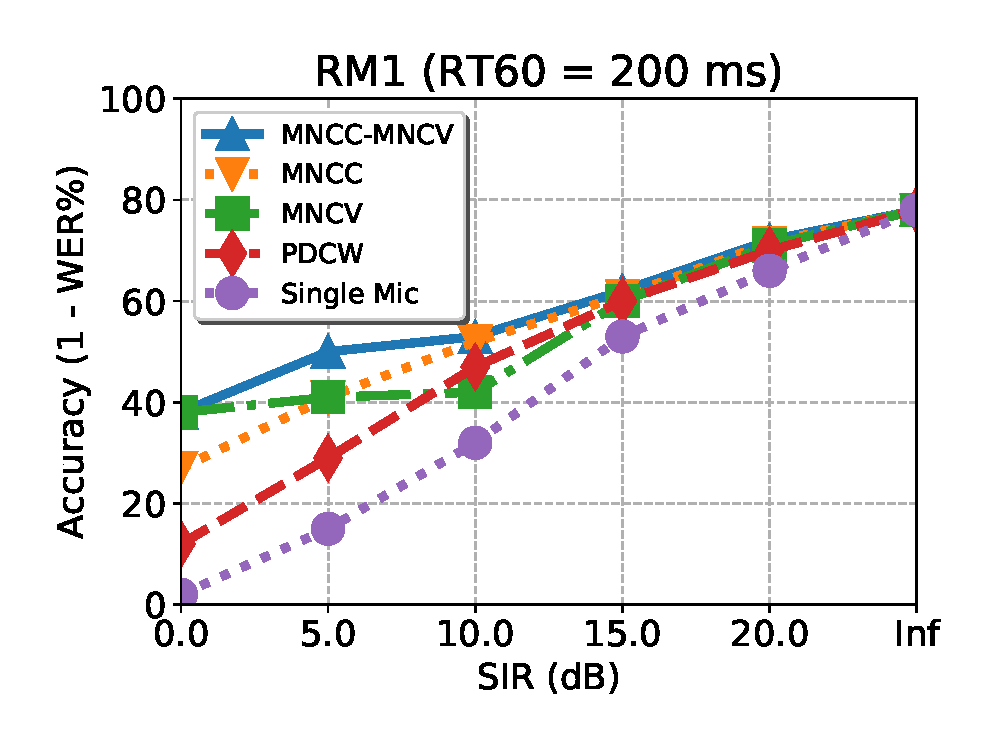
\includegraphics[width=65mm]{../figures/plot_mncc_mcc_wer_200ms}}   \vspace{-2mm} \\
           \subfigure[\label{fig:PDCW_AUTO_CorrTypes_Omni}]
           {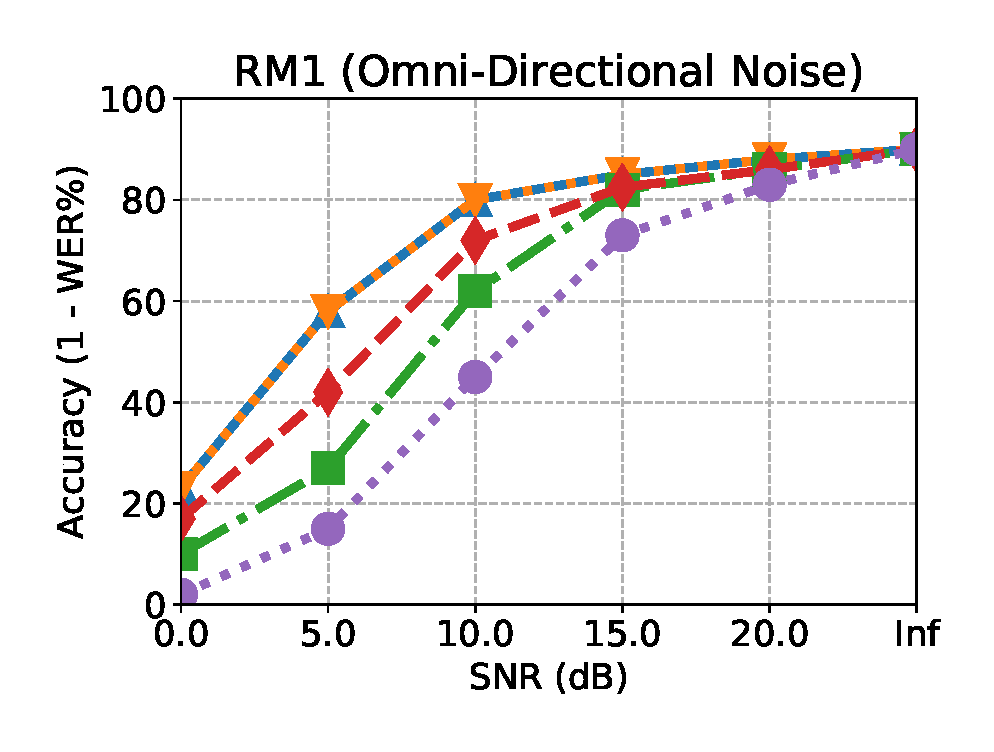
\includegraphics[width=65mm]{../figures/plot_mncc_mcc_wer_omni}}
          \vspace{-2mm}%
  %    \end{tabular}
       {\caption{\label{fig:PDCW_AUTO_CorrTypes_IntSNR}
             \emph{Comparison of recognition accuracy for the DARPA RM database (a) corrupted by an interfering speaker located at 30 degrees under the reverberation of $T_{60} = 200 ms $, and (b) in the presence of natural real-world noise.}
   }}
   \end{center}
   \vspace{-8mm}
\end{figure}
%
%
%
We determine which element
of this set is the most appropriate IMD threshold by performing an exhaustive search over the set $\mathcal{T}$. Let us consider one element of this set, $\tau_0 =   d \sin(\theta_{0}) f_s / c$.
%But these masks are two noisy too be directly used, so we need to use some smoothing in the frequency domain.
%For smoothing method, we can consider the gammatone channel weighting approach \cite{C_Kim_ASRU_2009_2}
%\cite{C_Kim_INTERSPEECH_2009_1} or simple smoothing across frequency indexes.
%The following is one example of obtaining smoothed mask
Using the procedure described in Sec. \ref{sec:sourceSeparation}, we obtain the target spectrum $X_T[m, e^{j \omega_k} | \tau_0], \quad 0 \le k \le \frac{K}{2}$  as shown below:
\begin{align}
        X_T[m, e^{j \omega_k} | \tau_0] = X_{A}[m, e^{j \omega_k}] \mu[m, k | \tau_0]
\end{align}
where $X_{A}[m, e^{j \omega_k}]$ is the averaged signal spectrogram from the two microphones defined by
\begin{equation}
  X_{A}[m,  e^{j \omega_k}] = (X_L[m, e^{j \omega_k} ]  + X_R[m, e^{j
  \omega_k}])/2.
\end{equation}
$\mu[m, k | \tau_0]$ is the binary mask obtained by \eqref{eq:decCriterionTau}.
In the above equation we explicitly include $\tau_0$ to show that the masked spectrum depends on
the IMD threshold. Using this spectrum $X_T[m, e^{j \omega_k}]$, we obtain the target power
and the power of the interfering sources. Since everything which is not the target is considered to be an interfering source,
the power associated with the target and interfering sources can be obtained by the following equations:
\begin{subequations}
    \begin{align}
    P_T[m|\tau_0] & =  \sum_{k=0}^{K-1} \Big|X_T[m, e^{j \omega_k} | \tau_0]\Big|^2 \\
    P_I[m|\tau_0] & =  \sum_{k=0}^{K-1} \Big|X_{A}[m, e^{j \omega_k}]\Big|^2 - P_T[m|\tau_0]
     \end{align}
     \label{P_TandP_I}
\end{subequations}
 As in \cite{C_Kim_INTERSPEECH_2010_1, C_Kim_IEEETran_2016_1, C_Kim_ICASSP_2012_1}, a compressive nonlinearity is invoked:
 \begin{subequations}
\begin{align}
    R_T[m|\tau_0]  =  P_T[m|\tau_0] ^ {a_0}  \qquad    R_I[m|\tau_0]  =  P_I[m|\tau_0] ^ {a_0}
\end{align}
 \label{NonlinearityOuput}
\end{subequations}
where   $a_0 = 1 / 15$ is the power coefficient as in
\cite{C_Kim_INTERSPEECH_2010_1, C_Kim_IEEETran_2016_1}.

In general, the optimal IMD threshold is determined by identifying the value of $\tau_0$ that minimizes the cross-correlation between the signals $R_T[m|\tau_0]$ and $R_I[m|\tau_0]$ from  \eqref{NonlinearityOuput}, but there are several plausible ways of computing this cross-correlation.  The first method considered, which was used in an earlier paper \cite{C_Kim_INTERSPEECH_2010_1}, is based on 
the normalized cross-covariance of the signals in  \eqref{NonlinearityOuput}:
\begin{align}
    \rho_{T,I}(\tau_0) = \frac{\frac{1}{K}\sum_{m=1}^{M} R_T[m|\tau_0]  R_I[m|\tau_0] - \mu_{R_T}\mu_{R_I}}{\sigma_{R_T} \sigma_{R_I}}
    \label{eq:TypeI}
\end{align}
where $\mu_{R_1}$ and $\mu_{R_2}$, and $\sigma_{R_T}$ and $\sigma_{R_I}$, are the means and standard deviations of $R_T[m|\tau_0]$ and $R_I[m|\tau_0]$, respectively.  (This statistic   is also known as the Pearson product-moment correlation.) 

The optimal IMD threshold $\tau_0$ is selected to minimize the absolute value
of the cross-covariance:
\begin{align}
    \hat{\tau}_1 = \arg \min_{\tau_0} |\rho_{T,I}(\tau_0)| \label{eq:minCrossCor}
\end{align}
 Again, we refer to this approach
as the MNCV statistic, and 
  it has provided good speech recognition accuracy as shown in Fig. \ref{fig:PDCW_AUTO_CorrTypes_IntSNR}, especially at low SNRs such as 0 or 5 dB. Nevertheless, at moderate SNRs such 10   or 15 dB, the speech recognition accuracies obtained using MNCV processing are   worse than those obtained using the PDCW algorithm.  MNCC-MNCV processing using the MNCV statistic also provides poor recognition accuracy in the presence of omnidirectional 
natural noise, as   shown in Fig. \ref{fig:PDCW_AUTO_CorrTypes_Omni}. 
We have also found in pilot studies that the MNCV statistic in  \eqref{eq:TypeI} is not a helpful measure in situations where there is a single interfering source with power that is comparable to that of the target, or where there are multiple interfering sources.  

To address this problem, we consider a second related statistic,    the   normalized cross-correlation:
\begin{align}
    r_{T,I}(\tau_0)  = \frac{\frac{1}{K}\sum_{m=1}^{M} R_T[m|\tau_0]  R_I[m|\tau_0]}{\sigma_{R_T} \sigma_{R_I}} \\
    \hat{\tau}_2  = \arg \min_{\tau_0} | r_{T,I}(\tau_0) |
\end{align}
We refer to implementations using $\hat{\tau}_2$   as Minimum Normalized Cross-correlation (MNCC) systems.
 
The final IMD threshold  $\hat{\tau}_3$ is obtained easily by calculating the minimum of $\hat{\tau}_1$ and $\hat{\tau}_2$ as shown below:
\begin{align}
    \hat{\tau}_3 = \min(\hat{\tau}_1, \hat{\tau}_2) 
    \label{eq:tau3_eq}
\end{align}
We refer to implementations using $\hat{\tau}_3$   as  MNCC-MNCV systems.
As can be seen in Figs. \ref{fig:PDCW_AUTO_CorrTypes_IntSNR}($a$) and \ref{fig:PDCW_AUTO_CorrTypes_Omni}, systems using the MNCC-MNCV
stastistic consistently provide recognition accuracy that is similar to or better than that obtained using either the     MNCV or MNCC approaches.  For these reasons we adopt MNCC-MNCV processing as the default approach, unless some other approach is stated explicitly. 
Instead of directly applying the mask $\mu[m, k | \hat{\tau}_3]$, 
we obtain a smoothed mask $\mu_s[m, k| \hat{\tau}_3]$ using the Channel Weighting
(CW) technique in \cite{C_Kim_INTERSPEECH_2009_1}. By applying $\mu_s[m, k| \hat{\tau}_3]$ to the averaged spectrum $X_{A}[m, e^{j \omega_k}]$, we obtain the enhanced spectrum $Y[m, e^{j \omega_k}]$ as follows:
\begin{align}
        Y[m, e^{j \omega_k}]= X_{A}[m, e^{j \omega_k}] \mu_s[m, k| \hat{\tau}_3]
\end{align}
% The reconstructed spectrum is given by:
%\begin{align}
%   Y [m, e^{j \omega k})  = \max\left[\mu_s[m, k], \eta\right] \, X_{A} [m, e^{j \omega k}),
%                         \; 0 \le k \le \frac{N}{2} \label{XcmResyn}
%\end{align}
%where again  we use $\eta=0.01$ as in \cite{C_Kim_INTERSPEECH_2009_1}, and $X_{A} [m, e^{j \omega k})$ is the averaged
%spectrum defined in  \eqref{eq:averageSpec}.
%In the discussion up to now  we have considered spectral components for frequency indicies $0 \le k \le \frac{N}{2} $. For $\frac{N}{2} + 1 \le k \le N - 1$, we obtain $X_T [m, e^{j \omega k} | \hat{\tau}_3)$ using the Hermition symmetry property of Fourier transforms of real time functions.  [THIS IS NOT SO IMPORTANT AND COMMONLY USED IN ANY CASE]
%
%\vspace{-2mm}
\subsection{Spectral flooring}
\label{sec:spectral_flooring}
%\vspace{-2mm}
%
In our previous work (\emph{e.g.}  \cite{C_Kim_IEEETran_2016_1} ), it has been frequently observed that an appropriate flooring helps in improving 
  noise robustness. For this reason we also
apply a flooring level to the spectrum, which is described by the   equation:
\begin{align}
Y_{f} = \delta_f \sqrt{\frac{1}{N_f K}  \sum_{m=0}^{N_f - 1} \sum_{k = 0}^{K - 1}  \big|Y[m, e^{j \omega_k}]\big|^2 }
\end{align}
where $\delta_f$ is the flooring coefficient, $N_f$ is the number of frames in the utterance,  $K$
is the FFT size, and $Y_{f}$ is the obtained threshold. We use a value of 0.01 for the flooring
coefficient $\delta_f$.
Using the flooring level $Y_{f}$, the floored spectrum $Z [m, e^{j \omega k}], 0 \le k \le K$ is obtained as follows:
	\begin{align}
    Z[m, e^{j \omega k}] =  \max\left[  \big| Y[m, e^{j \omega_k}] \big|
     , Y_f\right] e^ {j \angle Y[m, e^{j \omega_k}] }
	\end{align}
%The above equations mean that the magnitude spectrum is floored by a minimum value of $Y_f$ while 
 % the phase remains unchanged. 
Using $Z [m, e^{j \omega k}]$, speech is resynthesized using IFFT and the
overlap-add method (OLA). While the improved threshold optimization 
criteria in Sec. \ref{sec:optimalIMDthresholdSelection} is the most important 
improvement over our previous approach in \cite{C_Kim_INTERSPEECH_2010_1},
Channel Weighting (CW) and this spectral flooring are also additional
improvements.
%%
%\begin{figure}
%       \begin{center}
%          {\includegraphics[width=65mm]{../figures/PDCW_AUTO_CorrTypes_Omni_ICASSP}}  
%           \vspace{-6mm}%
%       {\caption{\label{fig:PDCW_AUTO_CorrTypes_Omni}
%            Speech recognition accuracy obtained using different algorithms in the presence of natural real-world noise.  \vspace{-6mm}%
%   }}
%   \end{center}
%\end{figure}
%%
\begin{figure}
       \begin{center}
    %   \begin{tabular}{c c c}
      \subfigure[\label{fig:PDCW_AUTO_IntSNR_Rev_0ms_Angle_30}]
           {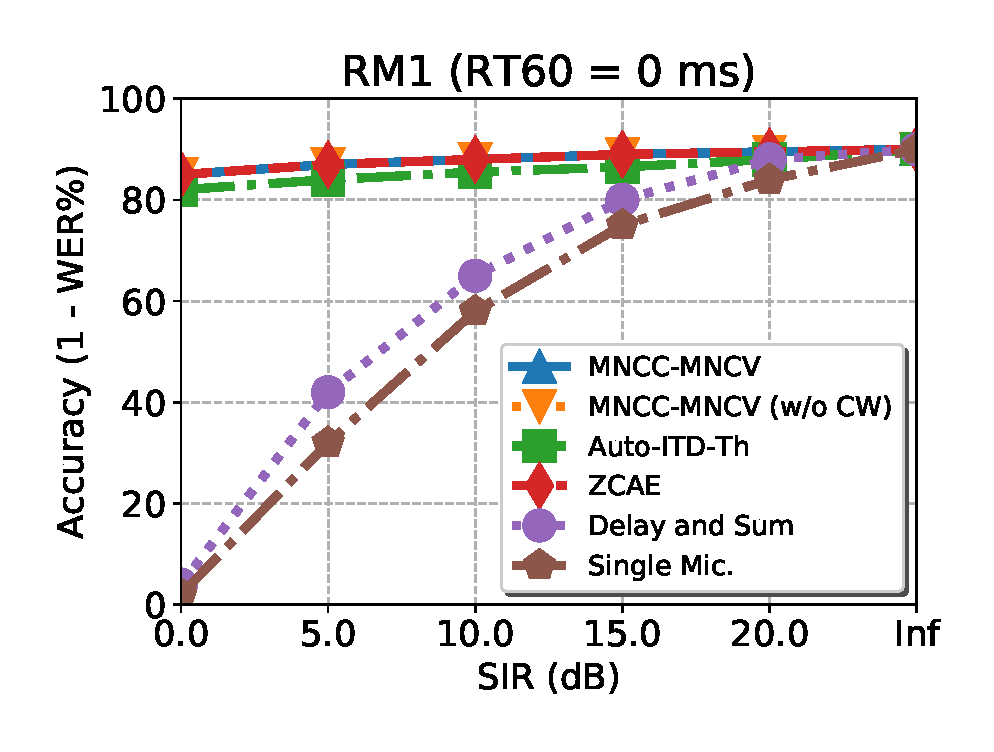
\includegraphics[width=65mm]{../figures/plot_comparison_0ms.eps}
           }
           \vspace{-2mm}
      %      \subfigure[\label{fig:PDCW_AUTO_IntSNR_Rev_100ms_Angle_30}]
     %     {\includegraphics[width=65mm]{../figures/PDCW_AUTO_IntSNR_Rev_100ms_Angle_30_ICASSP}} &
           \subfigure[\label{fig:PDCW_AUTO_IntSNR_Rev_200ms_Angle_30}]
           {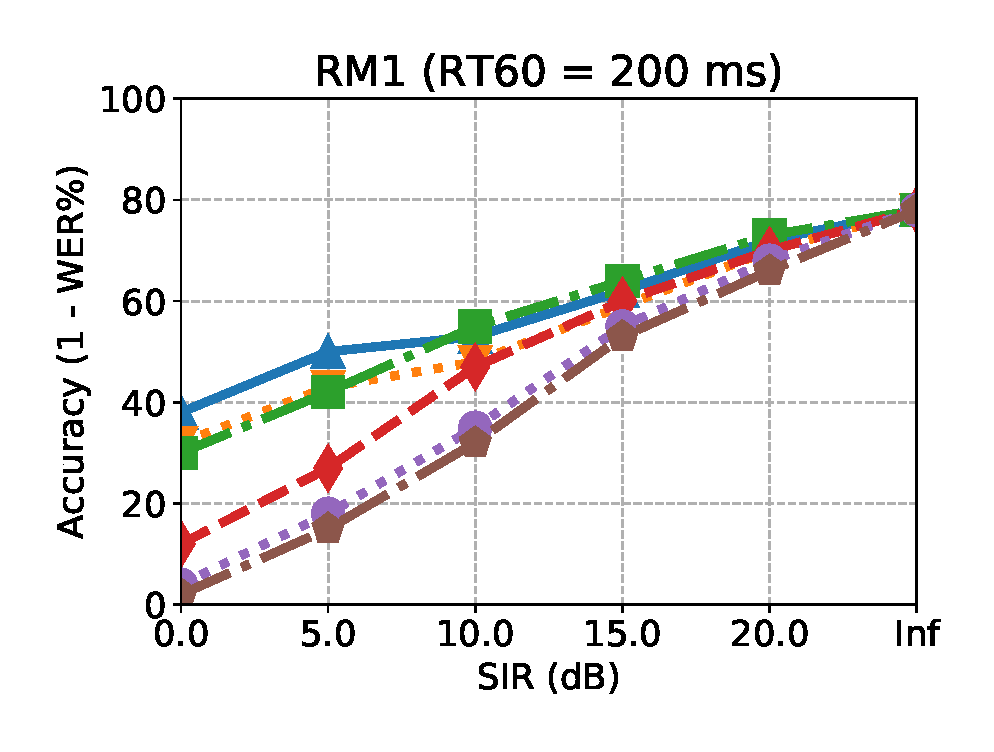
\includegraphics[width=65mm]{../figures/plot_comparison_200ms.eps}}
           \vspace{-2mm}
            \subfigure[\label{fig:ATIS_PDCW_PD_AUTO_FIXED_Omni}]
           {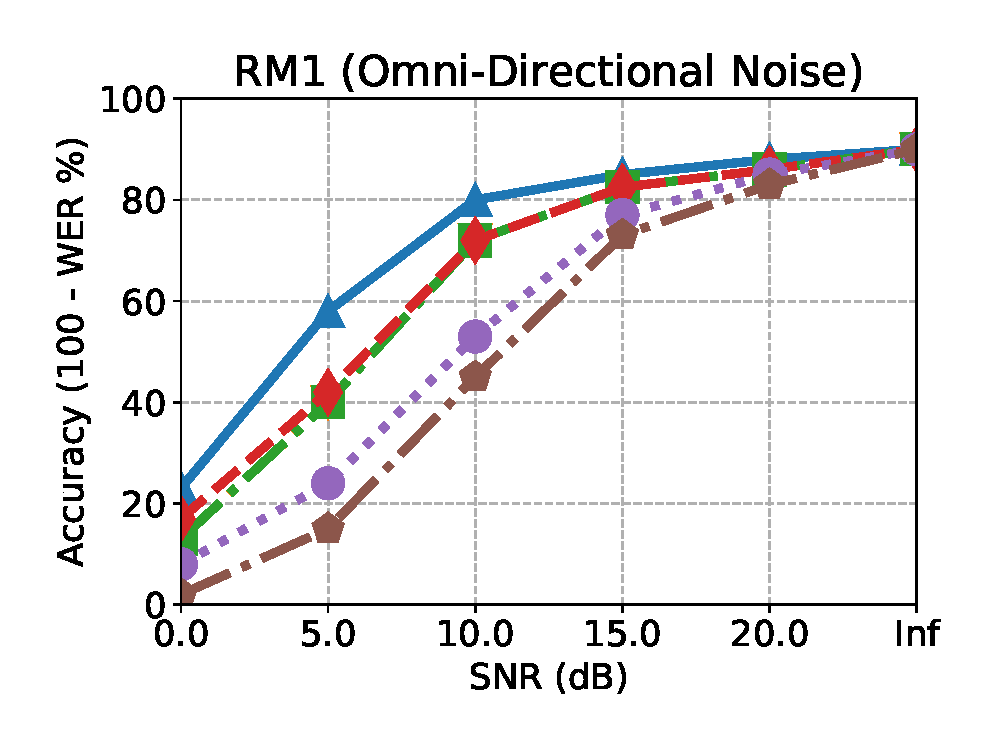
\includegraphics[width=65mm]{../figures/plot_comparison_omni.eps}}
          \vspace{-2mm}
    %  \end{tabular}
       {\caption{\label{fig:PDCW_AUTO_IntSNR}
        \emph{Comparison of recognition accuracy for the DARPA RM database (a) corrupted by an interfering speaker located at 30 degrees, (b) corrupted by an interfering speaker located at 30 degrees under the reverberation of $T_{60} = 200   $ ms, and (c) in the presence of natural real-world noise.}    
   }}
   \end{center}
   \vspace{-8mm}
\end{figure}
%
\begin{figure}
       \begin{center}
     %  \begin{tabular}{c c c}
         % \subfigure[\label{fig:PDCW_AUTO_IntLoc_Rev_0ms_Angle_45}]
         % {\includegraphics[width=65mm]{../figures/PDCW_AUTO_IntLoc_Rev_0ms_Angle_45_ICASSP}}   \vspace{-3mm} \\
       %     \subfigure[\label{fig:PDCW_AUTO_IntLoc_Rev_100ms_Angle_45}]
         {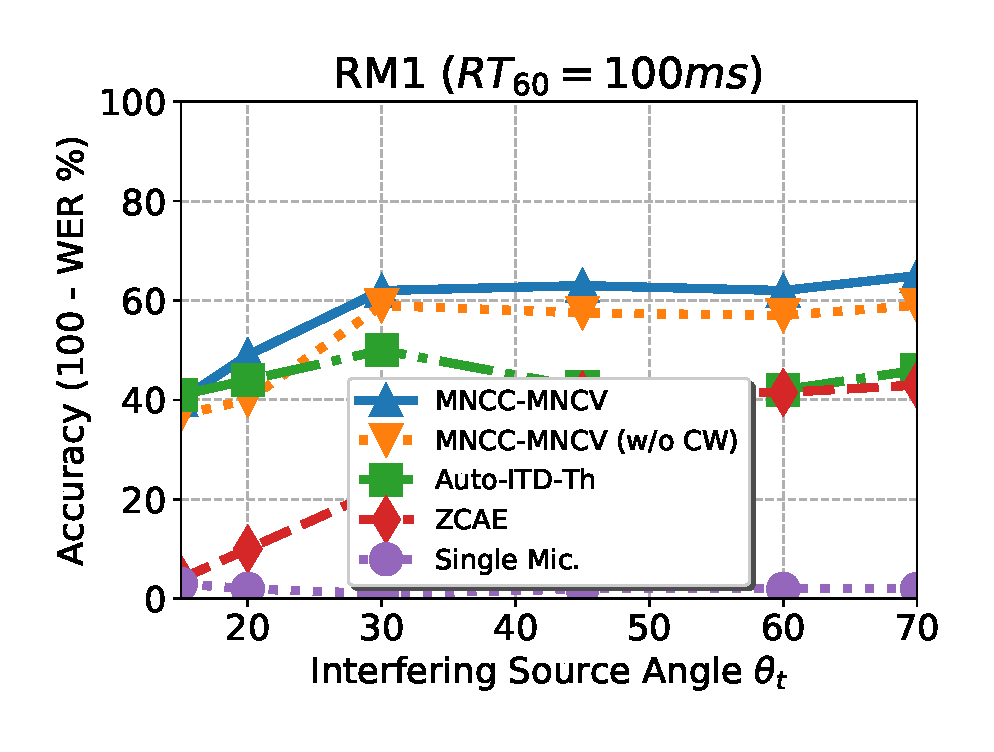
\includegraphics[width=65mm]{../figures/plot_comparison_angle}}
      %    \subfigure[\label{fig:PDCW_AUTO_IntLoc_Rev_200ms_Angle_45}]
      %    {\includegraphics[width=65mm]{../figures/PDCW_AUTO_IntLoc_Rev_200ms_Angle_45_ICASSP}} 
          % \vspace{-6mm}
    %  \end{tabular}
       {\caption{\label{fig:PDCW_AUTO_IntLoc}
                \emph{Comparison of recognition accuracy for the DARPA RM database corrupted by an interfering speaker   at different locations in a simulated room with 100 {\it ms} different reverberation time. (SIR) is fixed at 0 dB. } 
	       }}
   \end{center}
   \vspace{-8mm}
\end{figure}
%%%%%%%%%%%%%%%%%%%%%%%%%%%%%%%%%%%%%%%%%%%%%%%%%%%%%%%%%%%%%%%%%%%%%%%%
%
%  Section:	 Experimental results
%
%\vspace{-2mm}
\section{Experimental results}
%\vspace{-2mm}
	\label{sec:experimentalResults}
In this section, we present experimental results using the MNCC-MNCV algorithms 
described in this paper, focussing on the performance of the new methods that
were developed to estimate blindly the IMD threshold parameter. To evaluate the
effectiveness of this MNCC-MNCV algorithm, we performed
comparison with the source separation algorithm developed in  \cite
{C_Kim_INTERSPEECH_2010_1}, which is referred to as 
``Auto-ITD-Th" in this section. To see the additional benefit of Channel
Weighting (CW), we also compared the performance
when the Channel Weighting (CW) approach is not employed in
MNCC-MCVN.

 We also  compare our approach with an earlier  technique, the ZCAE algorithm
 described in  \cite{H_Park_SpeechComm_2009} 
using binary masking as in \cite{C_Kim_INTERSPEECH_2010_1}. In all speech recognition experiments described in this paper we perform feature extraction using  the version of MFCC processing implemented in  \texttt{sphinx\_fe} in \texttt{sphinxbase 0.4.1}.
For acoustic model training, we used \texttt{SphinxTrain 1.0}, and decoding was
performed using the  \texttt{CMU Sphinx 3.8}, all of which are readily available in Open Source form.
 We used subsets of 1600 utterances and 600 utterances, respectively, from the DARPA Resource Management (RM1) database for training and testing.
A bigram language model was used in all experiments. In all experiments, we used feature vectors
of length of 39 including delta and delta-delta features. We assumed that the distance between two microphones is 4 cm.

We conducted three different sets of experiments in this section.
The first two sets of experiments involve   simulated reverberant environments in which the target speaker is
masked by a single interfering speaker. 
 The reverberation simulations were accomplished using the \emph{Room Impulse Response} open source software package \cite{RIR} based on the image method.
   In these experiments, we assume a room of
dimensions 5 m x 4 m x 3 m, with microphones that are located at the center of the room.
Both the target and interfering sources are 1.5 m away from the microphone.
For the ZCAE algorithm, we used a threshold angle of  $\theta_{TH} = 20 ^ {\circ}$.

In the first set of experiments, we assume that the target is located along the perpendicular bisector of the 
line between two microphones, which means $\theta_T = 0^{\circ}$. We assume
that the interfering source is located at $\theta_I = 30^{\circ}$. We repeated the
experiments by changing the Signal-to-Interference Ratio (SIR) and reverberation time.
As shown in Fig. \ref{fig:PDCW_AUTO_IntSNR_Rev_0ms_Angle_30}, in the absence of
reverberation at 0-dB SIR, both the fixed-IMD system (ZCAE) and the automatic-IMD
systems (MNCC-MCNV, Auto-ITD-Th) provide comparable performance.   If   reverberation is present, however, 
MNCC-MNCV provides substantially better performance than the ZCAE signal separation system. 
In the second set of the experiments we changed the location of the interfering speaker while maintaining
the SIR   at 0 dB. As shown in Fig. \ref{fig:PDCW_AUTO_IntLoc}, even if the SIR is the same as in the calibration environment,
the performance of the fixed-IMD threshold system (ZCAE) becomes significantly degraded   if the actual interfering speaker
location is different from the location used in the calibration environment.   The MNCC-MNCV selection system
provides recognition results that are much more robust with respect to the locations of the interfering sources compared to ZCAE and the basic MNCC-MNCV/Auto-ITD-Th algorithm described in \cite{C_Kim_INTERSPEECH_2010_1}.  %Based on the results of Fig. 2 we believe that the differences between the results obtained with the 

 % In this figure we observe that as the interfering speaker moves
%toward the target,  the fixed-IMD threshold PD system provides   increased word error rate. %We repeated
%this   experiment with different reverberation times. As shown in Fig. \ref{fig:PDCW_AUTO_IntLoc}, the automatic-threshold-selection algorithm provides %consistently
%better recognition accuracy than the fixed threshold system, as expected. 
%
%
%\begin{figure}
%   \begin{center}
%            {\includegraphics[width=65mm]{../figures/ATIS_PDCW_PD_AUTO_FIXED_Omni_ICASSP}}           
%   \end{center}
%    \vspace{-6mm}%
%         {\caption{\label{fig:ATIS_PDCW_PD_AUTO_FIXED_Omni}
%         Speech recognition accuracy using different algorithms in the presence of natural real-world noise.       }
%    \vspace{-6mm}
%     }  
%\end{figure}
%
%
In the third set of experiments we added noise recorded with two microphones in real environments  such as a public  market, a food court,   a city street and a bus stop.  These real noise sources surround the two microphones, and the signals from these recordings are digitally added to clean speech from the   test set of the RM database.  Fig.
\ref{fig:ATIS_PDCW_PD_AUTO_FIXED_Omni} shows speech recognition accuracy for this configuration. 
Again we observe that  MNCC-MNCV provides the best performance by a significant
margin, while the  Auto-ITD-Th, MNCC-MCNV without CW, and ZCAE show similar performance to each other.
%
%In this paper, we conducted experiments in various configurations, and we observed that MNCC-MNCV provides significant 
%improvement in speech recognition accuracy for speech in various types of interfering noise sources and reverberation, compared to state-of-the-art algorithms that rely on a fixed IMD threshold.  The use of the automatic IMD threshold selection is particularly helpful in the presence of multiple interfering sources or reverberation, or when the location of the target source is not estimated properly.
%
\section{Summary}
 In this paper, we present a two-microphone algorithm for sound source separation 
    referred to as Minimum Normalized Cross-Correlation and Minimum Normalized 
    Cross-coVariance (MNCC-MNCV).  
We demonstrate that the use of the MNCC-MNCV method of estimating IMD
    thresholds  provides significantly better recognition accuracy in the
    presence of   interfering speech sources, omni-directional noise, and
    reverberation than several other approaches including ZCAE
    \cite{H_Park_SpeechComm_2009}, PDCW \cite{C_Kim_INTERSPEECH_2009_1}, and
    our previous automatic IMD threshold selection approach
    \cite{C_Kim_INTERSPEECH_2010_1}. 
% While the PDCW algorithm itself is not patent protected, a US patent has been applied for the automatic IMD threshold selection algorithm.
%
%
%\section{Summary}
%
%In this paper we introduce power-normalized cepstral coefficients (PNCC), which we characterize as a feature set that provides better recognition accuracy than MFCC and RASTA-PLP processing in the presence of common types of additive noise and reverberation.  PNCC processing is motivated by the desire to develop computationally efficient feature extraction for automatic speech recognition that is based on a pragmatic abstraction of various attributes of auditory processing including the rate-level nonlinearity, temporal and spectral integration, and temporal masking.  The processing also includes a
%component that implements suppression of various types of common additive noise.
%Further details about the motivation for and implementation of PNCC processing are available in \cite{ChanwooKimPhDThesis, C_Kim_IEEETran_2016_1}.
%This thesis also includes additional relevant experimental findings including results obtained for PNCC processing using multi-style training 
%and in combination  with speaker-by-speaker MLLR.
%Open Source MATLAB code for PNCC may be found at
%{\small\texttt{http://www.cs.cmu.edu/ \\
%\ \ \~{}robust/archive/algorithms/PNCC\_IEEETran}}.  The code in this directory was used for obtaining the results for this paper.
%
%
%  \newpage
 % \eightpt
\bibliographystyle{IEEEtran}
   %  \bibliographystyle{IEEEbib}
%
\bibliography{../../common_bib_file/common_bib_file}
%
%
%
%  \begin{thebibliography}{9}
%    \bibitem[1]{Davis80-COP}
%      S.\ B.\ Davis and P.\ Mermelstein,
%      ``Comparison of parametric representation for monosyllabic word recognition in continuously spoken sentences,''
%      \textit{IEEE Transactions on Acoustics, Speech and Signal Processing}, vol.~28, no.~4, pp.~357--366, 1980.
%    \bibitem[2]{Rabiner89-ATO}
%      L.\ R.\ Rabiner,
%      ``A tutorial on hidden Markov models and selected applications in speech recognition,''
%      \textit{Proceedings of the IEEE}, vol.~77, no.~2, pp.~257-286, 1989.
%    \bibitem[3]{Hastie09-TEO}
%      T.\ Hastie, R.\ Tibshirani, and J.\ Friedman,
%      \textit{The Elements of Statistical Learning -- Data Mining, Inference, and Prediction}.
%      New York: Springer, 2009.
%    \bibitem[4]{YourName15-XXX}
%      F.\ Lastname1, F.\ Lastname2, and F.\ Lastname3,
%      ``Title of your INTERSPEECH 2015 publication,''
%      in \textit{Interspeech 2015 -- 16\textsuperscript{th} Annual Conference of the International Speech Communication Association, September 06--10, Dresden, Germany, Proceedings}, 2015, pp.~100--104.
%  \end{thebibliography}

\end{document}
